% Created by tikzDevice version 0.10.1 on 2017-10-30 17:28:43
% !TEX encoding = UTF-8 Unicode
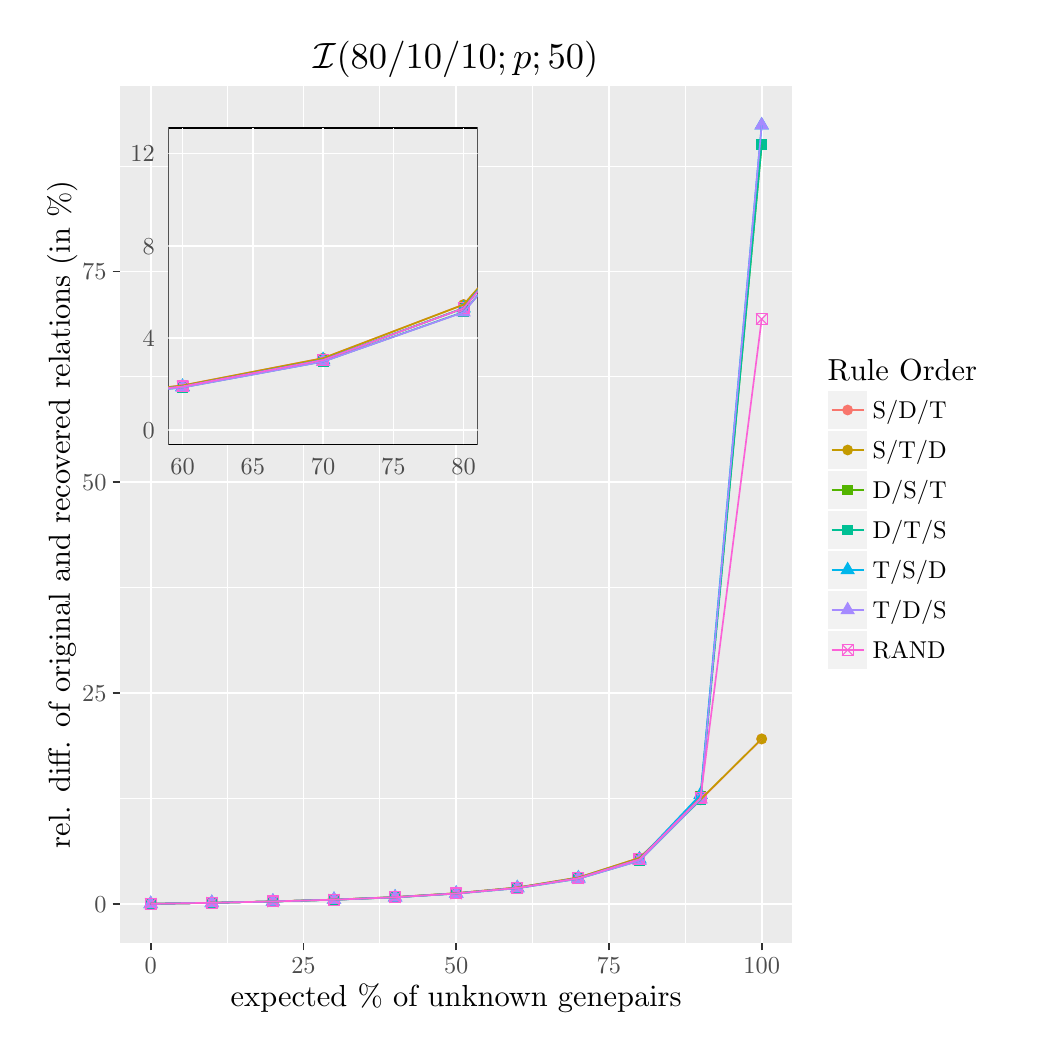
\begin{tikzpicture}[x=1pt,y=1pt]
\definecolor{fillColor}{RGB}{255,255,255}
\path[use as bounding box,fill=fillColor,fill opacity=0.00] (0,0) rectangle (361.35,361.35);
\begin{scope}
\path[clip] (  0.00,  0.00) rectangle (361.35,361.35);
\definecolor{drawColor}{RGB}{255,255,255}
\definecolor{fillColor}{RGB}{255,255,255}

\path[draw=drawColor,line width= 0.6pt,line join=round,line cap=round,fill=fillColor] (  0.00,  0.00) rectangle (361.35,361.35);
\end{scope}
\begin{scope}
\path[clip] ( 33.42, 30.69) rectangle (276.26,340.16);
\definecolor{fillColor}{gray}{0.92}

\path[fill=fillColor] ( 33.42, 30.69) rectangle (276.26,340.16);
\definecolor{drawColor}{RGB}{255,255,255}

\path[draw=drawColor,line width= 0.3pt,line join=round] ( 33.42, 82.83) --
	(276.26, 82.83);

\path[draw=drawColor,line width= 0.3pt,line join=round] ( 33.42,159.00) --
	(276.26,159.00);

\path[draw=drawColor,line width= 0.3pt,line join=round] ( 33.42,235.16) --
	(276.26,235.16);

\path[draw=drawColor,line width= 0.3pt,line join=round] ( 33.42,311.32) --
	(276.26,311.32);

\path[draw=drawColor,line width= 0.3pt,line join=round] ( 72.06, 30.69) --
	( 72.06,340.16);

\path[draw=drawColor,line width= 0.3pt,line join=round] (127.25, 30.69) --
	(127.25,340.16);

\path[draw=drawColor,line width= 0.3pt,line join=round] (182.44, 30.69) --
	(182.44,340.16);

\path[draw=drawColor,line width= 0.3pt,line join=round] (237.63, 30.69) --
	(237.63,340.16);

\path[draw=drawColor,line width= 0.6pt,line join=round] ( 33.42, 44.75) --
	(276.26, 44.75);

\path[draw=drawColor,line width= 0.6pt,line join=round] ( 33.42,120.92) --
	(276.26,120.92);

\path[draw=drawColor,line width= 0.6pt,line join=round] ( 33.42,197.08) --
	(276.26,197.08);

\path[draw=drawColor,line width= 0.6pt,line join=round] ( 33.42,273.24) --
	(276.26,273.24);

\path[draw=drawColor,line width= 0.6pt,line join=round] ( 44.46, 30.69) --
	( 44.46,340.16);

\path[draw=drawColor,line width= 0.6pt,line join=round] ( 99.65, 30.69) --
	( 99.65,340.16);

\path[draw=drawColor,line width= 0.6pt,line join=round] (154.84, 30.69) --
	(154.84,340.16);

\path[draw=drawColor,line width= 0.6pt,line join=round] (210.03, 30.69) --
	(210.03,340.16);

\path[draw=drawColor,line width= 0.6pt,line join=round] (265.23, 30.69) --
	(265.23,340.16);
\definecolor{fillColor}{RGB}{248,118,109}

\path[fill=fillColor] ( 44.46, 44.75) circle (  1.96);

\path[fill=fillColor] ( 66.54, 45.13) circle (  1.96);

\path[fill=fillColor] ( 88.61, 45.63) circle (  1.96);

\path[fill=fillColor] (110.69, 46.27) circle (  1.96);

\path[fill=fillColor] (132.77, 47.19) circle (  1.96);

\path[fill=fillColor] (154.84, 48.59) circle (  1.96);

\path[fill=fillColor] (176.92, 50.66) circle (  1.96);

\path[fill=fillColor] (199.00, 54.26) circle (  1.96);

\path[fill=fillColor] (221.07, 61.34) circle (  1.96);

\path[fill=fillColor] (243.15, 82.31) circle (  1.96);

\path[fill=fillColor] (265.23,104.34) circle (  1.96);
\definecolor{fillColor}{RGB}{196,154,0}

\path[fill=fillColor] ( 44.46, 44.75) circle (  1.96);

\path[fill=fillColor] ( 66.54, 45.12) circle (  1.96);

\path[fill=fillColor] ( 88.61, 45.62) circle (  1.96);

\path[fill=fillColor] (110.69, 46.27) circle (  1.96);

\path[fill=fillColor] (132.77, 47.18) circle (  1.96);

\path[fill=fillColor] (154.84, 48.58) circle (  1.96);

\path[fill=fillColor] (176.92, 50.64) circle (  1.96);

\path[fill=fillColor] (199.00, 54.25) circle (  1.96);

\path[fill=fillColor] (221.07, 61.34) circle (  1.96);

\path[fill=fillColor] (243.15, 82.50) circle (  1.96);

\path[fill=fillColor] (265.23,104.34) circle (  1.96);
\definecolor{fillColor}{RGB}{83,180,0}

\path[fill=fillColor] ( 42.50, 42.79) --
	( 46.42, 42.79) --
	( 46.42, 46.72) --
	( 42.50, 46.72) --
	cycle;

\path[fill=fillColor] ( 64.58, 43.16) --
	( 68.50, 43.16) --
	( 68.50, 47.08) --
	( 64.58, 47.08) --
	cycle;

\path[fill=fillColor] ( 86.65, 43.65) --
	( 90.58, 43.65) --
	( 90.58, 47.58) --
	( 86.65, 47.58) --
	cycle;

\path[fill=fillColor] (108.73, 44.29) --
	(112.65, 44.29) --
	(112.65, 48.21) --
	(108.73, 48.21) --
	cycle;

\path[fill=fillColor] (130.81, 45.17) --
	(134.73, 45.17) --
	(134.73, 49.10) --
	(130.81, 49.10) --
	cycle;

\path[fill=fillColor] (152.88, 46.56) --
	(156.81, 46.56) --
	(156.81, 50.49) --
	(152.88, 50.49) --
	cycle;

\path[fill=fillColor] (174.96, 48.57) --
	(178.88, 48.57) --
	(178.88, 52.50) --
	(174.96, 52.50) --
	cycle;

\path[fill=fillColor] (197.03, 52.06) --
	(200.96, 52.06) --
	(200.96, 55.98) --
	(197.03, 55.98) --
	cycle;

\path[fill=fillColor] (219.11, 58.91) --
	(223.03, 58.91) --
	(223.03, 62.84) --
	(219.11, 62.84) --
	cycle;

\path[fill=fillColor] (241.19, 81.60) --
	(245.11, 81.60) --
	(245.11, 85.53) --
	(241.19, 85.53) --
	cycle;

\path[fill=fillColor] (263.26,317.05) --
	(267.19,317.05) --
	(267.19,320.97) --
	(263.26,320.97) --
	cycle;
\definecolor{fillColor}{RGB}{0,192,148}

\path[fill=fillColor] ( 42.50, 42.79) --
	( 46.42, 42.79) --
	( 46.42, 46.72) --
	( 42.50, 46.72) --
	cycle;

\path[fill=fillColor] ( 64.58, 43.15) --
	( 68.50, 43.15) --
	( 68.50, 47.08) --
	( 64.58, 47.08) --
	cycle;

\path[fill=fillColor] ( 86.65, 43.64) --
	( 90.58, 43.64) --
	( 90.58, 47.56) --
	( 86.65, 47.56) --
	cycle;

\path[fill=fillColor] (108.73, 44.26) --
	(112.65, 44.26) --
	(112.65, 48.19) --
	(108.73, 48.19) --
	cycle;

\path[fill=fillColor] (130.81, 45.12) --
	(134.73, 45.12) --
	(134.73, 49.05) --
	(130.81, 49.05) --
	cycle;

\path[fill=fillColor] (152.88, 46.49) --
	(156.81, 46.49) --
	(156.81, 50.41) --
	(152.88, 50.41) --
	cycle;

\path[fill=fillColor] (174.96, 48.43) --
	(178.88, 48.43) --
	(178.88, 52.36) --
	(174.96, 52.36) --
	cycle;

\path[fill=fillColor] (197.03, 51.85) --
	(200.96, 51.85) --
	(200.96, 55.77) --
	(197.03, 55.77) --
	cycle;

\path[fill=fillColor] (219.11, 58.40) --
	(223.03, 58.40) --
	(223.03, 62.33) --
	(219.11, 62.33) --
	cycle;

\path[fill=fillColor] (241.19, 80.45) --
	(245.11, 80.45) --
	(245.11, 84.37) --
	(241.19, 84.37) --
	cycle;

\path[fill=fillColor] (263.26,317.05) --
	(267.19,317.05) --
	(267.19,320.97) --
	(263.26,320.97) --
	cycle;
\definecolor{fillColor}{RGB}{0,182,235}

\path[fill=fillColor] ( 44.46, 47.80) --
	( 47.10, 43.23) --
	( 41.82, 43.23) --
	cycle;

\path[fill=fillColor] ( 66.54, 48.17) --
	( 69.18, 43.59) --
	( 63.90, 43.59) --
	cycle;

\path[fill=fillColor] ( 88.61, 48.66) --
	( 91.26, 44.09) --
	( 85.97, 44.09) --
	cycle;

\path[fill=fillColor] (110.69, 49.30) --
	(113.33, 44.72) --
	(108.05, 44.72) --
	cycle;

\path[fill=fillColor] (132.77, 50.19) --
	(135.41, 45.61) --
	(130.12, 45.61) --
	cycle;

\path[fill=fillColor] (154.84, 51.56) --
	(157.49, 46.99) --
	(152.20, 46.99) --
	cycle;

\path[fill=fillColor] (176.92, 53.56) --
	(179.56, 48.98) --
	(174.28, 48.98) --
	cycle;

\path[fill=fillColor] (199.00, 57.09) --
	(201.64, 52.51) --
	(196.35, 52.51) --
	cycle;

\path[fill=fillColor] (221.07, 63.92) --
	(223.72, 59.35) --
	(218.43, 59.35) --
	cycle;

\path[fill=fillColor] (243.15, 87.26) --
	(245.79, 82.68) --
	(240.51, 82.68) --
	cycle;

\path[fill=fillColor] (265.23,329.14) --
	(267.87,324.57) --
	(262.58,324.57) --
	cycle;
\definecolor{fillColor}{RGB}{165,138,255}

\path[fill=fillColor] ( 44.46, 47.80) --
	( 47.10, 43.23) --
	( 41.82, 43.23) --
	cycle;

\path[fill=fillColor] ( 66.54, 48.17) --
	( 69.18, 43.59) --
	( 63.90, 43.59) --
	cycle;

\path[fill=fillColor] ( 88.61, 48.65) --
	( 91.26, 44.07) --
	( 85.97, 44.07) --
	cycle;

\path[fill=fillColor] (110.69, 49.28) --
	(113.33, 44.70) --
	(108.05, 44.70) --
	cycle;

\path[fill=fillColor] (132.77, 50.14) --
	(135.41, 45.56) --
	(130.12, 45.56) --
	cycle;

\path[fill=fillColor] (154.84, 51.50) --
	(157.49, 46.92) --
	(152.20, 46.92) --
	cycle;

\path[fill=fillColor] (176.92, 53.43) --
	(179.56, 48.85) --
	(174.28, 48.85) --
	cycle;

\path[fill=fillColor] (199.00, 56.85) --
	(201.64, 52.27) --
	(196.35, 52.27) --
	cycle;

\path[fill=fillColor] (221.07, 63.38) --
	(223.72, 58.80) --
	(218.43, 58.80) --
	cycle;

\path[fill=fillColor] (243.15, 85.64) --
	(245.79, 81.06) --
	(240.51, 81.06) --
	cycle;

\path[fill=fillColor] (265.23,329.14) --
	(267.87,324.57) --
	(262.58,324.57) --
	cycle;
\definecolor{drawColor}{RGB}{251,97,215}

\path[draw=drawColor,line width= 0.4pt,line join=round,line cap=round] ( 42.50, 42.79) rectangle ( 46.42, 46.72);

\path[draw=drawColor,line width= 0.4pt,line join=round,line cap=round] ( 42.50, 42.79) -- ( 46.42, 46.72);

\path[draw=drawColor,line width= 0.4pt,line join=round,line cap=round] ( 42.50, 46.72) -- ( 46.42, 42.79);

\path[draw=drawColor,line width= 0.4pt,line join=round,line cap=round] ( 64.58, 43.16) rectangle ( 68.50, 47.08);

\path[draw=drawColor,line width= 0.4pt,line join=round,line cap=round] ( 64.58, 43.16) -- ( 68.50, 47.08);

\path[draw=drawColor,line width= 0.4pt,line join=round,line cap=round] ( 64.58, 47.08) -- ( 68.50, 43.16);

\path[draw=drawColor,line width= 0.4pt,line join=round,line cap=round] ( 86.65, 43.65) rectangle ( 90.58, 47.57);

\path[draw=drawColor,line width= 0.4pt,line join=round,line cap=round] ( 86.65, 43.65) -- ( 90.58, 47.57);

\path[draw=drawColor,line width= 0.4pt,line join=round,line cap=round] ( 86.65, 47.57) -- ( 90.58, 43.65);

\path[draw=drawColor,line width= 0.4pt,line join=round,line cap=round] (108.73, 44.29) rectangle (112.65, 48.21);

\path[draw=drawColor,line width= 0.4pt,line join=round,line cap=round] (108.73, 44.29) -- (112.65, 48.21);

\path[draw=drawColor,line width= 0.4pt,line join=round,line cap=round] (108.73, 48.21) -- (112.65, 44.29);

\path[draw=drawColor,line width= 0.4pt,line join=round,line cap=round] (130.81, 45.18) rectangle (134.73, 49.10);

\path[draw=drawColor,line width= 0.4pt,line join=round,line cap=round] (130.81, 45.18) -- (134.73, 49.10);

\path[draw=drawColor,line width= 0.4pt,line join=round,line cap=round] (130.81, 49.10) -- (134.73, 45.18);

\path[draw=drawColor,line width= 0.4pt,line join=round,line cap=round] (152.88, 46.54) rectangle (156.81, 50.46);

\path[draw=drawColor,line width= 0.4pt,line join=round,line cap=round] (152.88, 46.54) -- (156.81, 50.46);

\path[draw=drawColor,line width= 0.4pt,line join=round,line cap=round] (152.88, 50.46) -- (156.81, 46.54);

\path[draw=drawColor,line width= 0.4pt,line join=round,line cap=round] (174.96, 48.56) rectangle (178.88, 52.49);

\path[draw=drawColor,line width= 0.4pt,line join=round,line cap=round] (174.96, 48.56) -- (178.88, 52.49);

\path[draw=drawColor,line width= 0.4pt,line join=round,line cap=round] (174.96, 52.49) -- (178.88, 48.56);

\path[draw=drawColor,line width= 0.4pt,line join=round,line cap=round] (197.03, 52.05) rectangle (200.96, 55.98);

\path[draw=drawColor,line width= 0.4pt,line join=round,line cap=round] (197.03, 52.05) -- (200.96, 55.98);

\path[draw=drawColor,line width= 0.4pt,line join=round,line cap=round] (197.03, 55.98) -- (200.96, 52.05);

\path[draw=drawColor,line width= 0.4pt,line join=round,line cap=round] (219.11, 58.89) rectangle (223.03, 62.82);

\path[draw=drawColor,line width= 0.4pt,line join=round,line cap=round] (219.11, 58.89) -- (223.03, 62.82);

\path[draw=drawColor,line width= 0.4pt,line join=round,line cap=round] (219.11, 62.82) -- (223.03, 58.89);

\path[draw=drawColor,line width= 0.4pt,line join=round,line cap=round] (241.19, 81.18) rectangle (245.11, 85.11);

\path[draw=drawColor,line width= 0.4pt,line join=round,line cap=round] (241.19, 81.18) -- (245.11, 85.11);

\path[draw=drawColor,line width= 0.4pt,line join=round,line cap=round] (241.19, 85.11) -- (245.11, 81.18);

\path[draw=drawColor,line width= 0.4pt,line join=round,line cap=round] (263.26,254.09) rectangle (267.19,258.02);

\path[draw=drawColor,line width= 0.4pt,line join=round,line cap=round] (263.26,254.09) -- (267.19,258.02);

\path[draw=drawColor,line width= 0.4pt,line join=round,line cap=round] (263.26,258.02) -- (267.19,254.09);
\definecolor{drawColor}{RGB}{248,118,109}

\path[draw=drawColor,line width= 0.6pt,line join=round] ( 44.46, 44.75) --
	( 66.54, 45.13) --
	( 88.61, 45.63) --
	(110.69, 46.27) --
	(132.77, 47.19) --
	(154.84, 48.59) --
	(176.92, 50.66) --
	(199.00, 54.26) --
	(221.07, 61.34) --
	(243.15, 82.31) --
	(265.23,104.34);
\definecolor{drawColor}{RGB}{196,154,0}

\path[draw=drawColor,line width= 0.6pt,line join=round] ( 44.46, 44.75) --
	( 66.54, 45.12) --
	( 88.61, 45.62) --
	(110.69, 46.27) --
	(132.77, 47.18) --
	(154.84, 48.58) --
	(176.92, 50.64) --
	(199.00, 54.25) --
	(221.07, 61.34) --
	(243.15, 82.50) --
	(265.23,104.34);
\definecolor{drawColor}{RGB}{83,180,0}

\path[draw=drawColor,line width= 0.6pt,line join=round] ( 44.46, 44.75) --
	( 66.54, 45.12) --
	( 88.61, 45.61) --
	(110.69, 46.25) --
	(132.77, 47.13) --
	(154.84, 48.53) --
	(176.92, 50.53) --
	(199.00, 54.02) --
	(221.07, 60.87) --
	(243.15, 83.57) --
	(265.23,319.01);
\definecolor{drawColor}{RGB}{0,192,148}

\path[draw=drawColor,line width= 0.6pt,line join=round] ( 44.46, 44.75) --
	( 66.54, 45.12) --
	( 88.61, 45.60) --
	(110.69, 46.22) --
	(132.77, 47.09) --
	(154.84, 48.45) --
	(176.92, 50.39) --
	(199.00, 53.81) --
	(221.07, 60.36) --
	(243.15, 82.41) --
	(265.23,319.01);
\definecolor{drawColor}{RGB}{0,182,235}

\path[draw=drawColor,line width= 0.6pt,line join=round] ( 44.46, 44.75) --
	( 66.54, 45.12) --
	( 88.61, 45.61) --
	(110.69, 46.25) --
	(132.77, 47.14) --
	(154.84, 48.51) --
	(176.92, 50.51) --
	(199.00, 54.04) --
	(221.07, 60.87) --
	(243.15, 84.21) --
	(265.23,326.09);
\definecolor{drawColor}{RGB}{165,138,255}

\path[draw=drawColor,line width= 0.6pt,line join=round] ( 44.46, 44.75) --
	( 66.54, 45.11) --
	( 88.61, 45.60) --
	(110.69, 46.23) --
	(132.77, 47.09) --
	(154.84, 48.45) --
	(176.92, 50.38) --
	(199.00, 53.80) --
	(221.07, 60.33) --
	(243.15, 82.58) --
	(265.23,326.09);
\definecolor{drawColor}{RGB}{251,97,215}

\path[draw=drawColor,line width= 0.6pt,line join=round] ( 44.46, 44.75) --
	( 66.54, 45.12) --
	( 88.61, 45.61) --
	(110.69, 46.25) --
	(132.77, 47.14) --
	(154.84, 48.50) --
	(176.92, 50.52) --
	(199.00, 54.01) --
	(221.07, 60.86) --
	(243.15, 83.14) --
	(265.23,256.05);
\end{scope}
\begin{scope}
\path[clip] (  0.00,  0.00) rectangle (361.35,361.35);
\definecolor{drawColor}{gray}{0.30}

\node[text=drawColor,anchor=base east,inner sep=0pt, outer sep=0pt, scale=  0.88] at ( 28.47, 41.72) {0};

\node[text=drawColor,anchor=base east,inner sep=0pt, outer sep=0pt, scale=  0.88] at ( 28.47,117.89) {25};

\node[text=drawColor,anchor=base east,inner sep=0pt, outer sep=0pt, scale=  0.88] at ( 28.47,194.05) {50};

\node[text=drawColor,anchor=base east,inner sep=0pt, outer sep=0pt, scale=  0.88] at ( 28.47,270.21) {75};
\end{scope}
\begin{scope}
\path[clip] (  0.00,  0.00) rectangle (361.35,361.35);
\definecolor{drawColor}{gray}{0.20}

\path[draw=drawColor,line width= 0.6pt,line join=round] ( 30.67, 44.75) --
	( 33.42, 44.75);

\path[draw=drawColor,line width= 0.6pt,line join=round] ( 30.67,120.92) --
	( 33.42,120.92);

\path[draw=drawColor,line width= 0.6pt,line join=round] ( 30.67,197.08) --
	( 33.42,197.08);

\path[draw=drawColor,line width= 0.6pt,line join=round] ( 30.67,273.24) --
	( 33.42,273.24);
\end{scope}
\begin{scope}
\path[clip] (  0.00,  0.00) rectangle (361.35,361.35);
\definecolor{drawColor}{gray}{0.20}

\path[draw=drawColor,line width= 0.6pt,line join=round] ( 44.46, 27.94) --
	( 44.46, 30.69);

\path[draw=drawColor,line width= 0.6pt,line join=round] ( 99.65, 27.94) --
	( 99.65, 30.69);

\path[draw=drawColor,line width= 0.6pt,line join=round] (154.84, 27.94) --
	(154.84, 30.69);

\path[draw=drawColor,line width= 0.6pt,line join=round] (210.03, 27.94) --
	(210.03, 30.69);

\path[draw=drawColor,line width= 0.6pt,line join=round] (265.23, 27.94) --
	(265.23, 30.69);
\end{scope}
\begin{scope}
\path[clip] (  0.00,  0.00) rectangle (361.35,361.35);
\definecolor{drawColor}{gray}{0.30}

\node[text=drawColor,anchor=base,inner sep=0pt, outer sep=0pt, scale=  0.88] at ( 44.46, 19.68) {0};

\node[text=drawColor,anchor=base,inner sep=0pt, outer sep=0pt, scale=  0.88] at ( 99.65, 19.68) {25};

\node[text=drawColor,anchor=base,inner sep=0pt, outer sep=0pt, scale=  0.88] at (154.84, 19.68) {50};

\node[text=drawColor,anchor=base,inner sep=0pt, outer sep=0pt, scale=  0.88] at (210.03, 19.68) {75};

\node[text=drawColor,anchor=base,inner sep=0pt, outer sep=0pt, scale=  0.88] at (265.23, 19.68) {100};
\end{scope}
\begin{scope}
\path[clip] (  0.00,  0.00) rectangle (361.35,361.35);
\definecolor{drawColor}{RGB}{0,0,0}

\node[text=drawColor,anchor=base,inner sep=0pt, outer sep=0pt, scale=  1.10] at (154.84,  7.70) {expected \% of unknown genepairs};
\end{scope}
\begin{scope}
\path[clip] (  0.00,  0.00) rectangle (361.35,361.35);
\definecolor{drawColor}{RGB}{0,0,0}

\node[text=drawColor,rotate= 90.00,anchor=base,inner sep=0pt, outer sep=0pt, scale=  1.10] at ( 15.28,185.42) {rel. diff. of original and recovered relations (in \%)};
\end{scope}
\begin{scope}
\path[clip] (  0.00,  0.00) rectangle (361.35,361.35);
\definecolor{fillColor}{RGB}{255,255,255}

\path[fill=fillColor] (284.80,124.97) rectangle (347.31,245.87);
\end{scope}
\begin{scope}
\path[clip] (  0.00,  0.00) rectangle (361.35,361.35);
\definecolor{drawColor}{RGB}{0,0,0}

\node[text=drawColor,anchor=base west,inner sep=0pt, outer sep=0pt, scale=  1.10] at (289.07,234.03) {Rule Order};
\end{scope}
\begin{scope}
\path[clip] (  0.00,  0.00) rectangle (361.35,361.35);
\definecolor{drawColor}{RGB}{255,255,255}
\definecolor{fillColor}{gray}{0.95}

\path[draw=drawColor,line width= 0.6pt,line join=round,line cap=round,fill=fillColor] (289.07,215.96) rectangle (303.52,230.42);
\end{scope}
\begin{scope}
\path[clip] (  0.00,  0.00) rectangle (361.35,361.35);
\definecolor{fillColor}{RGB}{248,118,109}

\path[fill=fillColor] (296.29,223.19) circle (  1.96);
\end{scope}
\begin{scope}
\path[clip] (  0.00,  0.00) rectangle (361.35,361.35);
\definecolor{drawColor}{RGB}{248,118,109}

\path[draw=drawColor,line width= 0.6pt,line join=round] (290.51,223.19) -- (302.08,223.19);
\end{scope}
\begin{scope}
\path[clip] (  0.00,  0.00) rectangle (361.35,361.35);
\definecolor{drawColor}{RGB}{255,255,255}
\definecolor{fillColor}{gray}{0.95}

\path[draw=drawColor,line width= 0.6pt,line join=round,line cap=round,fill=fillColor] (289.07,201.51) rectangle (303.52,215.96);
\end{scope}
\begin{scope}
\path[clip] (  0.00,  0.00) rectangle (361.35,361.35);
\definecolor{fillColor}{RGB}{196,154,0}

\path[fill=fillColor] (296.29,208.74) circle (  1.96);
\end{scope}
\begin{scope}
\path[clip] (  0.00,  0.00) rectangle (361.35,361.35);
\definecolor{drawColor}{RGB}{196,154,0}

\path[draw=drawColor,line width= 0.6pt,line join=round] (290.51,208.74) -- (302.08,208.74);
\end{scope}
\begin{scope}
\path[clip] (  0.00,  0.00) rectangle (361.35,361.35);
\definecolor{drawColor}{RGB}{255,255,255}
\definecolor{fillColor}{gray}{0.95}

\path[draw=drawColor,line width= 0.6pt,line join=round,line cap=round,fill=fillColor] (289.07,187.06) rectangle (303.52,201.51);
\end{scope}
\begin{scope}
\path[clip] (  0.00,  0.00) rectangle (361.35,361.35);
\definecolor{fillColor}{RGB}{83,180,0}

\path[fill=fillColor] (294.33,192.32) --
	(298.26,192.32) --
	(298.26,196.24) --
	(294.33,196.24) --
	cycle;
\end{scope}
\begin{scope}
\path[clip] (  0.00,  0.00) rectangle (361.35,361.35);
\definecolor{drawColor}{RGB}{83,180,0}

\path[draw=drawColor,line width= 0.6pt,line join=round] (290.51,194.28) -- (302.08,194.28);
\end{scope}
\begin{scope}
\path[clip] (  0.00,  0.00) rectangle (361.35,361.35);
\definecolor{drawColor}{RGB}{255,255,255}
\definecolor{fillColor}{gray}{0.95}

\path[draw=drawColor,line width= 0.6pt,line join=round,line cap=round,fill=fillColor] (289.07,172.60) rectangle (303.52,187.06);
\end{scope}
\begin{scope}
\path[clip] (  0.00,  0.00) rectangle (361.35,361.35);
\definecolor{fillColor}{RGB}{0,192,148}

\path[fill=fillColor] (294.33,177.87) --
	(298.26,177.87) --
	(298.26,181.79) --
	(294.33,181.79) --
	cycle;
\end{scope}
\begin{scope}
\path[clip] (  0.00,  0.00) rectangle (361.35,361.35);
\definecolor{drawColor}{RGB}{0,192,148}

\path[draw=drawColor,line width= 0.6pt,line join=round] (290.51,179.83) -- (302.08,179.83);
\end{scope}
\begin{scope}
\path[clip] (  0.00,  0.00) rectangle (361.35,361.35);
\definecolor{drawColor}{RGB}{255,255,255}
\definecolor{fillColor}{gray}{0.95}

\path[draw=drawColor,line width= 0.6pt,line join=round,line cap=round,fill=fillColor] (289.07,158.15) rectangle (303.52,172.60);
\end{scope}
\begin{scope}
\path[clip] (  0.00,  0.00) rectangle (361.35,361.35);
\definecolor{fillColor}{RGB}{0,182,235}

\path[fill=fillColor] (296.29,168.43) --
	(298.94,163.85) --
	(293.65,163.85) --
	cycle;
\end{scope}
\begin{scope}
\path[clip] (  0.00,  0.00) rectangle (361.35,361.35);
\definecolor{drawColor}{RGB}{0,182,235}

\path[draw=drawColor,line width= 0.6pt,line join=round] (290.51,165.37) -- (302.08,165.37);
\end{scope}
\begin{scope}
\path[clip] (  0.00,  0.00) rectangle (361.35,361.35);
\definecolor{drawColor}{RGB}{255,255,255}
\definecolor{fillColor}{gray}{0.95}

\path[draw=drawColor,line width= 0.6pt,line join=round,line cap=round,fill=fillColor] (289.07,143.69) rectangle (303.52,158.15);
\end{scope}
\begin{scope}
\path[clip] (  0.00,  0.00) rectangle (361.35,361.35);
\definecolor{fillColor}{RGB}{165,138,255}

\path[fill=fillColor] (296.29,153.97) --
	(298.94,149.39) --
	(293.65,149.39) --
	cycle;
\end{scope}
\begin{scope}
\path[clip] (  0.00,  0.00) rectangle (361.35,361.35);
\definecolor{drawColor}{RGB}{165,138,255}

\path[draw=drawColor,line width= 0.6pt,line join=round] (290.51,150.92) -- (302.08,150.92);
\end{scope}
\begin{scope}
\path[clip] (  0.00,  0.00) rectangle (361.35,361.35);
\definecolor{drawColor}{RGB}{255,255,255}
\definecolor{fillColor}{gray}{0.95}

\path[draw=drawColor,line width= 0.6pt,line join=round,line cap=round,fill=fillColor] (289.07,129.24) rectangle (303.52,143.69);
\end{scope}
\begin{scope}
\path[clip] (  0.00,  0.00) rectangle (361.35,361.35);
\definecolor{drawColor}{RGB}{251,97,215}

\path[draw=drawColor,line width= 0.4pt,line join=round,line cap=round] (294.33,134.50) rectangle (298.26,138.43);

\path[draw=drawColor,line width= 0.4pt,line join=round,line cap=round] (294.33,134.50) -- (298.26,138.43);

\path[draw=drawColor,line width= 0.4pt,line join=round,line cap=round] (294.33,138.43) -- (298.26,134.50);
\end{scope}
\begin{scope}
\path[clip] (  0.00,  0.00) rectangle (361.35,361.35);
\definecolor{drawColor}{RGB}{251,97,215}

\path[draw=drawColor,line width= 0.6pt,line join=round] (290.51,136.47) -- (302.08,136.47);
\end{scope}
\begin{scope}
\path[clip] (  0.00,  0.00) rectangle (361.35,361.35);
\definecolor{drawColor}{RGB}{0,0,0}

\node[text=drawColor,anchor=base west,inner sep=0pt, outer sep=0pt, scale=  0.88] at (305.33,220.16) {S/D/T};
\end{scope}
\begin{scope}
\path[clip] (  0.00,  0.00) rectangle (361.35,361.35);
\definecolor{drawColor}{RGB}{0,0,0}

\node[text=drawColor,anchor=base west,inner sep=0pt, outer sep=0pt, scale=  0.88] at (305.33,205.71) {S/T/D};
\end{scope}
\begin{scope}
\path[clip] (  0.00,  0.00) rectangle (361.35,361.35);
\definecolor{drawColor}{RGB}{0,0,0}

\node[text=drawColor,anchor=base west,inner sep=0pt, outer sep=0pt, scale=  0.88] at (305.33,191.25) {D/S/T};
\end{scope}
\begin{scope}
\path[clip] (  0.00,  0.00) rectangle (361.35,361.35);
\definecolor{drawColor}{RGB}{0,0,0}

\node[text=drawColor,anchor=base west,inner sep=0pt, outer sep=0pt, scale=  0.88] at (305.33,176.80) {D/T/S};
\end{scope}
\begin{scope}
\path[clip] (  0.00,  0.00) rectangle (361.35,361.35);
\definecolor{drawColor}{RGB}{0,0,0}

\node[text=drawColor,anchor=base west,inner sep=0pt, outer sep=0pt, scale=  0.88] at (305.33,162.34) {T/S/D};
\end{scope}
\begin{scope}
\path[clip] (  0.00,  0.00) rectangle (361.35,361.35);
\definecolor{drawColor}{RGB}{0,0,0}

\node[text=drawColor,anchor=base west,inner sep=0pt, outer sep=0pt, scale=  0.88] at (305.33,147.89) {T/D/S};
\end{scope}
\begin{scope}
\path[clip] (  0.00,  0.00) rectangle (361.35,361.35);
\definecolor{drawColor}{RGB}{0,0,0}

\node[text=drawColor,anchor=base west,inner sep=0pt, outer sep=0pt, scale=  0.88] at (305.33,133.44) {RAND};
\end{scope}
\begin{scope}
\path[clip] (  0.00,  0.00) rectangle (361.35,361.35);
\definecolor{drawColor}{RGB}{0,0,0}

\node[text=drawColor,anchor=base,inner sep=0pt, outer sep=0pt, scale=  1.32] at (154.84,346.76) {$\mathcal{I}(80/10/10;p;50)$};
\end{scope}
\begin{scope}
\path[clip] ( 54.20,216.81) rectangle (162.61,325.21);
\definecolor{drawColor}{RGB}{255,255,255}
\definecolor{fillColor}{RGB}{255,255,255}

\path[draw=drawColor,line width= 0.6pt,line join=round,line cap=round,fill=fillColor] ( 54.20,216.81) rectangle (162.61,325.21);
\end{scope}
\begin{scope}
\path[clip] ( 50.88,210.75) rectangle (162.61,325.21);
\definecolor{drawColor}{RGB}{0,0,0}
\definecolor{fillColor}{gray}{0.92}

\path[draw=drawColor,line width= 0.6pt,line join=round,line cap=round,fill=fillColor] ( 50.88,210.75) rectangle (162.61,325.21);
\definecolor{drawColor}{RGB}{255,255,255}

\path[draw=drawColor,line width= 0.6pt,line join=round] ( 50.88,215.95) --
	(162.61,215.95);

\path[draw=drawColor,line width= 0.6pt,line join=round] ( 50.88,249.25) --
	(162.61,249.25);

\path[draw=drawColor,line width= 0.6pt,line join=round] ( 50.88,282.55) --
	(162.61,282.55);

\path[draw=drawColor,line width= 0.6pt,line join=round] ( 50.88,315.85) --
	(162.61,315.85);

\path[draw=drawColor,line width= 0.6pt,line join=round] ( 55.96,210.75) --
	( 55.96,325.21);

\path[draw=drawColor,line width= 0.6pt,line join=round] ( 81.35,210.75) --
	( 81.35,325.21);

\path[draw=drawColor,line width= 0.6pt,line join=round] (106.74,210.75) --
	(106.74,325.21);

\path[draw=drawColor,line width= 0.6pt,line join=round] (132.14,210.75) --
	(132.14,325.21);

\path[draw=drawColor,line width= 0.6pt,line join=round] (157.53,210.75) --
	(157.53,325.21);
\definecolor{fillColor}{RGB}{248,118,109}

\path[fill=fillColor] (  5.17,226.43) circle (  1.96);

\path[fill=fillColor] ( 55.96,232.08) circle (  1.96);

\path[fill=fillColor] (106.74,241.93) circle (  1.96);

\path[fill=fillColor] (157.53,261.28) circle (  1.96);

\path[fill=fillColor] (208.31,318.59) circle (  1.96);
\definecolor{fillColor}{RGB}{196,154,0}

\path[fill=fillColor] (  5.17,226.41) circle (  1.96);

\path[fill=fillColor] ( 55.96,232.03) circle (  1.96);

\path[fill=fillColor] (106.74,241.89) circle (  1.96);

\path[fill=fillColor] (157.53,261.27) circle (  1.96);

\path[fill=fillColor] (208.31,319.10) circle (  1.96);
\definecolor{fillColor}{RGB}{83,180,0}

\path[fill=fillColor] (  3.21,224.30) --
	(  7.13,224.30) --
	(  7.13,228.22) --
	(  3.21,228.22) --
	cycle;

\path[fill=fillColor] ( 54.00,229.79) --
	( 57.92,229.79) --
	( 57.92,233.71) --
	( 54.00,233.71) --
	cycle;

\path[fill=fillColor] (104.78,239.31) --
	(108.71,239.31) --
	(108.71,243.23) --
	(104.78,243.23) --
	cycle;

\path[fill=fillColor] (155.57,258.04) --
	(159.49,258.04) --
	(159.49,261.96) --
	(155.57,261.96) --
	cycle;

\path[fill=fillColor] (206.35,320.05) --
	(210.28,320.05) --
	(210.28,323.97) --
	(206.35,323.97) --
	cycle;
\definecolor{fillColor}{RGB}{0,192,148}

\path[fill=fillColor] (  3.21,224.09) --
	(  7.13,224.09) --
	(  7.13,228.01) --
	(  3.21,228.01) --
	cycle;

\path[fill=fillColor] ( 54.00,229.40) --
	( 57.92,229.40) --
	( 57.92,233.33) --
	( 54.00,233.33) --
	cycle;

\path[fill=fillColor] (104.78,238.73) --
	(108.71,238.73) --
	(108.71,242.66) --
	(104.78,242.66) --
	cycle;

\path[fill=fillColor] (155.57,256.65) --
	(159.49,256.65) --
	(159.49,260.57) --
	(155.57,260.57) --
	cycle;

\path[fill=fillColor] (206.35,316.88) --
	(210.28,316.88) --
	(210.28,320.81) --
	(206.35,320.81) --
	cycle;
\definecolor{fillColor}{RGB}{0,182,235}

\path[fill=fillColor] (  5.17,229.27) --
	(  7.81,224.70) --
	(  2.53,224.70) --
	cycle;

\path[fill=fillColor] ( 55.96,234.72) --
	( 58.60,230.14) --
	( 53.31,230.14) --
	cycle;

\path[fill=fillColor] (106.74,244.38) --
	(109.39,239.80) --
	(104.10,239.80) --
	cycle;

\path[fill=fillColor] (157.53,263.05) --
	(160.17,258.47) --
	(154.89,258.47) --
	cycle;

\path[fill=fillColor] (208.31,326.82) --
	(210.96,322.24) --
	(205.67,322.24) --
	cycle;
\definecolor{fillColor}{RGB}{165,138,255}

\path[fill=fillColor] (  5.17,229.09) --
	(  7.81,224.52) --
	(  2.53,224.52) --
	cycle;

\path[fill=fillColor] ( 55.96,234.38) --
	( 58.60,229.80) --
	( 53.31,229.80) --
	cycle;

\path[fill=fillColor] (106.74,243.72) --
	(109.39,239.15) --
	(104.10,239.15) --
	cycle;

\path[fill=fillColor] (157.53,261.57) --
	(160.17,256.99) --
	(154.89,256.99) --
	cycle;

\path[fill=fillColor] (208.31,322.38) --
	(210.96,317.80) --
	(205.67,317.80) --
	cycle;
\definecolor{drawColor}{RGB}{251,97,215}

\path[draw=drawColor,line width= 0.4pt,line join=round,line cap=round] (  3.21,224.23) rectangle (  7.13,228.15);

\path[draw=drawColor,line width= 0.4pt,line join=round,line cap=round] (  3.21,224.23) -- (  7.13,228.15);

\path[draw=drawColor,line width= 0.4pt,line join=round,line cap=round] (  3.21,228.15) -- (  7.13,224.23);

\path[draw=drawColor,line width= 0.4pt,line join=round,line cap=round] ( 54.00,229.76) rectangle ( 57.92,233.68);

\path[draw=drawColor,line width= 0.4pt,line join=round,line cap=round] ( 54.00,229.76) -- ( 57.92,233.68);

\path[draw=drawColor,line width= 0.4pt,line join=round,line cap=round] ( 54.00,233.68) -- ( 57.92,229.76);

\path[draw=drawColor,line width= 0.4pt,line join=round,line cap=round] (104.78,239.29) rectangle (108.71,243.22);

\path[draw=drawColor,line width= 0.4pt,line join=round,line cap=round] (104.78,239.29) -- (108.71,243.22);

\path[draw=drawColor,line width= 0.4pt,line join=round,line cap=round] (104.78,243.22) -- (108.71,239.29);

\path[draw=drawColor,line width= 0.4pt,line join=round,line cap=round] (155.57,257.99) rectangle (159.49,261.91);

\path[draw=drawColor,line width= 0.4pt,line join=round,line cap=round] (155.57,257.99) -- (159.49,261.91);

\path[draw=drawColor,line width= 0.4pt,line join=round,line cap=round] (155.57,261.91) -- (159.49,257.99);

\path[draw=drawColor,line width= 0.4pt,line join=round,line cap=round] (206.35,318.89) rectangle (210.28,322.82);

\path[draw=drawColor,line width= 0.4pt,line join=round,line cap=round] (206.35,318.89) -- (210.28,322.82);

\path[draw=drawColor,line width= 0.4pt,line join=round,line cap=round] (206.35,322.82) -- (210.28,318.89);
\definecolor{drawColor}{RGB}{248,118,109}

\path[draw=drawColor,line width= 0.6pt,line join=round] (  0.00,226.04) --
	(  5.17,226.43) --
	( 55.96,232.08) --
	(106.74,241.93) --
	(157.53,261.28) --
	(208.31,318.59) --
	(244.40,361.35);
\definecolor{drawColor}{RGB}{196,154,0}

\path[draw=drawColor,line width= 0.6pt,line join=round] (  0.00,226.02) --
	(  5.17,226.41) --
	( 55.96,232.03) --
	(106.74,241.89) --
	(157.53,261.27) --
	(208.31,319.10) --
	(244.28,361.35);
\definecolor{drawColor}{RGB}{83,180,0}

\path[draw=drawColor,line width= 0.6pt,line join=round] (  0.00,225.87) --
	(  5.17,226.26) --
	( 55.96,231.75) --
	(106.74,241.27) --
	(157.53,260.00) --
	(208.31,322.01) --
	(211.42,361.35);
\definecolor{drawColor}{RGB}{0,192,148}

\path[draw=drawColor,line width= 0.6pt,line join=round] (  0.00,225.67) --
	(  5.17,226.05) --
	( 55.96,231.36) --
	(106.74,240.70) --
	(157.53,258.61) --
	(208.31,318.85) --
	(211.65,361.35);
\definecolor{drawColor}{RGB}{0,182,235}

\path[draw=drawColor,line width= 0.6pt,line join=round] (  0.00,225.84) --
	(  5.17,226.22) --
	( 55.96,231.67) --
	(106.74,241.33) --
	(157.53,260.00) --
	(208.31,323.77) --
	(211.20,361.35);
\definecolor{drawColor}{RGB}{165,138,255}

\path[draw=drawColor,line width= 0.6pt,line join=round] (  0.00,225.66) --
	(  5.17,226.04) --
	( 55.96,231.33) --
	(106.74,240.67) --
	(157.53,258.52) --
	(208.31,319.33) --
	(211.52,361.35);
\definecolor{drawColor}{RGB}{251,97,215}

\path[draw=drawColor,line width= 0.6pt,line join=round] (  0.00,225.81) --
	(  5.17,226.19) --
	( 55.96,231.72) --
	(106.74,241.25) --
	(157.53,259.95) --
	(208.31,320.85) --
	(212.67,361.35);
\end{scope}
\begin{scope}
\path[clip] (  0.00,  0.00) rectangle (361.35,361.35);
\definecolor{drawColor}{gray}{0.30}

\node[text=drawColor,anchor=base east,inner sep=0pt, outer sep=0pt, scale=  0.88] at ( 45.93,212.92) {0};

\node[text=drawColor,anchor=base east,inner sep=0pt, outer sep=0pt, scale=  0.88] at ( 45.93,246.22) {4};

\node[text=drawColor,anchor=base east,inner sep=0pt, outer sep=0pt, scale=  0.88] at ( 45.93,279.52) {8};

\node[text=drawColor,anchor=base east,inner sep=0pt, outer sep=0pt, scale=  0.88] at ( 45.93,312.82) {12};
\end{scope}
\begin{scope}
\path[clip] (  0.00,  0.00) rectangle (361.35,361.35);
\definecolor{drawColor}{gray}{0.30}

\node[text=drawColor,anchor=base,inner sep=0pt, outer sep=0pt, scale=  0.88] at ( 55.96,199.74) {60};

\node[text=drawColor,anchor=base,inner sep=0pt, outer sep=0pt, scale=  0.88] at ( 81.35,199.74) {65};

\node[text=drawColor,anchor=base,inner sep=0pt, outer sep=0pt, scale=  0.88] at (106.74,199.74) {70};

\node[text=drawColor,anchor=base,inner sep=0pt, outer sep=0pt, scale=  0.88] at (132.14,199.74) {75};

\node[text=drawColor,anchor=base,inner sep=0pt, outer sep=0pt, scale=  0.88] at (157.53,199.74) {80};
\end{scope}
\end{tikzpicture}
